\documentclass[10pt]{article}
\usepackage{amsmath,textcomp,amssymb,geometry,graphicx,enumerate,tikz,algorithm,algpseudocode,pifont,upgreek}
\usetikzlibrary{calc}
\usetikzlibrary{datavisualization}
\usetikzlibrary{datavisualization.formats.functions}


\textheight=9in
\textwidth=7in
\topmargin=-.75in
\oddsidemargin=-0.25in
\evensidemargin=-0.25in

\usepackage{listings}
\lstnewenvironment{codeblock}
    {\lstset{language=Python,
      showspaces=false,
      showtabs=false,
      breaklines=true,
      mathescape=true,
      showstringspaces=false,
      breakatwhitespace=true,
      commentstyle=\textit,
      keywordstyle=\textbf,
      basicstyle=\ttfamily,
      escapechar=`,
    }}
    {}

\newcommand{\bigo}{\mathcal{O}}
\newcommand{\R}{\mathbb{R}}


\begin{document}
\section*{04/18/2016}
\subsection*{Spectral Graph Clustering}
\begin{itemize}
	\item Input: Weighted, undirected graph $G = (V, E)$. No self-edges. $w_{ij} = $ weight of edge, $(i,j) = (j,i)$; zero if $(i,j)$ not in $E$.
	\item Goal: Cut $G$ into 2 (or more) pieces $G_{i}$ of similar sizes, but don't cut too much edge weight. e.g. Minimize the \underline{sparsity} $\frac{Cut(G_{1}, G_{2})}{Mass(G_{1}) \cdot Mass(G_{2})}$  aka \underline{cut ratio}, where $Cut(G_{1}, G_{2}) = $ total weight of cut edges, $Mass(G_{1}) = $\# of vertices in $G_{i}$ or assign masses to vertices.
		\begin{center}
			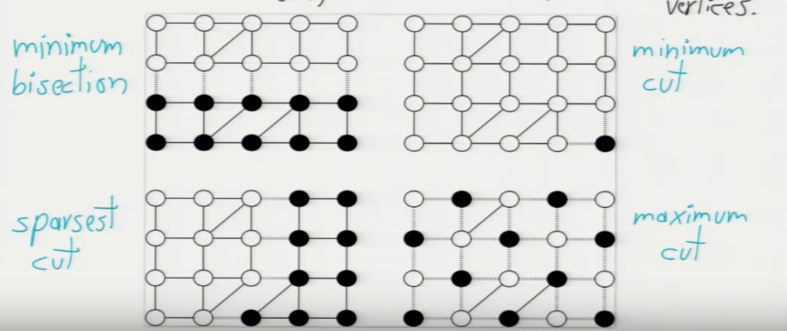
\includegraphics[scale=0.5]{../images/cuts}
		\end{center}
	\item Let $n = |V|$. Let $y \in \R^{n}$ be an \underline{indicator vector}:
			\[
 				y_{i} = \left\{\def\arraystretch{1.2}%
 				\begin{array}{@{}c@{\quad}l@{}}
    				1 & \text{vertex } i \in G_{1} \\
    				-1 & \text{vertex } i \in G_{2} \\
  				\end{array}\right.
			\]
			then 
			\[
 				\frac{w_{ij}}{4}(y_{i} - y_{j})^{2} = \left\{\def\arraystretch{1.2}%
 				\begin{array}{@{}c@{\quad}l@{}}
    				w_{ij} & (i, j) \text{ is a cut,} \\
    				0 & (i, j) \text{ is not a cut.} \\
  				\end{array}\right.
			\]
			\begin{align*}
				Cut(G_{1}, G_{2}) &= \sum_{(i,j) \in E} \frac{w_{ij}}{4}(y_{i} - y_{j})^{2}\\
				&= \frac{1}{4} \sum_{(i,j) \in E} (w_{ij}y_{i}^{2} - 2w_{ij}y_{i}y_{j} + w_{ij}y_{j}^{2})\\
				&= \frac{1}{4}\bigg(\sum_{(i,j) \in E} -2w_{ij}y_{i}y_{j} + \sum_{i=1}^{n} y_{i}^{2} \sum_{k\neq i}w_{ik}\bigg)\\
				&= \frac{y^{T}Ly}{4}\\
			\end{align*} 
			where,
			\[
 				L_{ij} = \left\{\def\arraystretch{1.2}%
 				\begin{array}{@{}c@{\quad}l@{}}
    				-w_{ij} & i \neq j \\
    				\sum_{k\neq i} w_{ik} & i = j \\
  				\end{array}\right.
			\]
			
		\item $L$ is symmetric, $n-$by$-n$ \underline{Laplacian matrix} for $G$.
			\begin{center}
				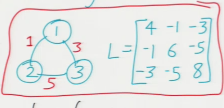
\includegraphics{../images/cutexample}
			\end{center}
		\item If $y = \begin{bmatrix}
			1 & 1& 1 & \dots & 1
		\end{bmatrix}^{T}$, then $Cut(G_{1}, G_{2}) = 0$ 1 is an eigenvector of $L$ w/eigenvalue 0.
		\item \underline{Bisection}: exactly $\frac{n}{2}$ vertices in $G_{1}$, $\frac{n}{2}$ in $G_{2}$. Write $\textbf{1}^{T}y = 0$.
		\begin{center}
			\begin{tabular}{|c|}
				\hline
				Find $y$ that minimizes $y^{T}Ly$ s.t. $\forall i, \ y_{i} = 1 or y_{i} = -1$ and $\textbf{1}^{T}y =0$\\
				\hline
			\end{tabular}
		\end{center}
	\item NP-hard. We \underline{relax} the binary constraint $\rightarrow$ fractional vertices.
	\item New constraint: $y$ must lie on sphere of radius $\sqrt{n}$.
	\item Relaxed problem:
		\begin{center}
			\begin{tabular}{|c|}
				\hline
				Minimize $y^{T}Ly$ s.t. $y^{T}y = n$ and $\textbf{1}^{T}y = 0$\\
				\hline
			\end{tabular}
		\end{center}
		\begin{center}
			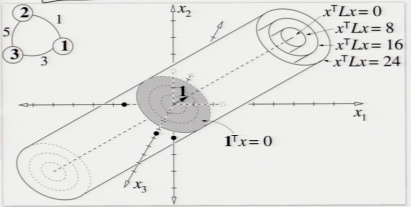
\includegraphics{../images/relaxed}
			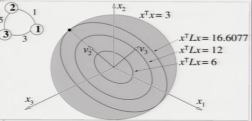
\includegraphics{../images/sphere}
		\end{center}
	\item Let $\lambda_{2} =$ second-smallest eigenvalue of $L$.
	\item Eigenvector $v_{2}$ is the \underline{fiedler vector}.	
	\item Spectral partitioning algorithm:
		\begin{itemize}
			\item Compute Fiedler vector $v_{2}$ of $L$.
			\item Round $v_{2}$ with a \underline{sweep cut}:
				\begin{itemize}
					\item Sort components of $v_{2}$
					\item Try the $n-1$ cuts between successive components.
					\item Choose sparsest cut.
				\end{itemize}
		\end{itemize}
	\item Fact: Sweep cut finds a cut w/sparsity $\leq \sqrt{2\lambda_{2} \ \max_{i} \frac{L_{ii}}{M_{ii}}}$.
	\item \underline{Cheeger's inequality}.
	\item The optimal cut has sparsity $\geq \frac{\lambda_{2}}{2}$.
\end{itemize}

	\subsubsection*{Vertex Masses}
	\begin{itemize}
		\item Let $M$ be a diagonal matrix w/vertex masses on diagonal.
		\item New balance constraint: $\textbf{1}^{T}My = 0$
		\item New ellipsoid constraint: $y^{T}My = Mass(G) = \sum_{i}M_{ii}$.
		\begin{center}
			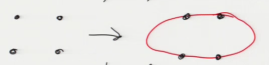
\includegraphics{../images/toellipsoid}
		\end{center}
		\item Now we want Fiedler vector of \underline{generalized eigensystem} $Lv = \lambda Mv$.
	\end{itemize}
	
	\subsubsection*{Greedy Divisive Clustering}
	\begin{itemize}
		\item Partition $G$ into 2 subgraphs; recursively cluster them.
		\item Can form a dendogram, but it may have inversions.
	\end{itemize}
	\subsubsection*{The Normalized Cut}
	\begin{itemize}
		\item Set vertex i's mass $M_{ii} = L_{ii}$.
		\item Popular for \underline{image segmentation}.
		\item For pixels with location $w_{i}$, brightness $b_{i}$
			\begin{align*}
				w_{ij} = exp\bigg(\frac{-|w_{i} - w_{j}|^{2}}{\alpha} - \frac{|b_{i} - b_{j}|^{2}}{\beta}\bigg)
			\end{align*}
			or zero if $|w_{i} - w_{j}|$ large.
	\end{itemize}
\end{document}










